% Für Bindekorrektur als optionales Argument "BCORfaktormitmaßeinheit", dann
% sieht auch Option "twoside" vernünftig aus
% Näheres zu "scrartcl" bzw. "scrreprt" und "scrbook" siehe KOMA-Skript Doku
\documentclass[12pt,a4paper,titlepage,headinclude,bibtotoc]{scrartcl}


%---- Allgemeine Layout Einstellungen ------------------------------------------

% Für Kopf und Fußzeilen, siehe auch KOMA-Skript Doku
\usepackage[komastyle]{scrpage2}
\pagestyle{scrheadings}
\setheadsepline{0.5pt}[\color{black}]
\automark[section]{chapter}


%Einstellungen für Figuren- und Tabellenbeschriftungen
\setkomafont{captionlabel}{\sffamily\bfseries}
\setcapindent{0em}


%---- Weitere Pakete -----------------------------------------------------------
% Die Pakete sind alle in der TeX Live Distribution enthalten. Wichtige Adressen
% www.ctan.org, www.dante.de

% Sprachunterstützung
\usepackage[ngerman]{babel}

% Benutzung von Umlauten direkt im Text
% entweder "latin1" oder "utf8"
\usepackage[utf8]{inputenc}

% Pakete mit Mathesymbolen und zur Beseitigung von Schwächen der Mathe-Umgebung
\usepackage{latexsym,exscale,stmaryrd,amssymb,amsmath}

% Weitere Symbole
\usepackage[nointegrals]{wasysym}
\usepackage{eurosym}

% Anderes Literaturverzeichnisformat
%\usepackage[square,sort&compress]{natbib}

% Für Farbe
\usepackage{color}

% Zur Graphikausgabe
%Beipiel: \includegraphics[width=\textwidth]{grafik.png}
\usepackage{graphicx}

% Text umfließt Graphiken und Tabellen
% Beispiel:
% \begin{wrapfigure}[Zeilenanzahl]{"l" oder "r"}{breite}
%   \centering
%   \includegraphics[width=...]{grafik}
%   \caption{Beschriftung} 
%   \label{fig:grafik}
% \end{wrapfigure}
\usepackage{wrapfig}

% Mehrere Abbildungen nebeneinander
% Beispiel:
% \begin{figure}[htb]
%   \centering
%   \subfigure[Beschriftung 1\label{fig:label1}]
%   {\includegraphics[width=0.49\textwidth]{grafik1}}
%   \hfill
%   \subfigure[Beschriftung 2\label{fig:label2}]
%   {\includegraphics[width=0.49\textwidth]{grafik2}}
%   \caption{Beschriftung allgemein}
%   \label{fig:label-gesamt}
% \end{figure}
\usepackage{subfigure}

% Caption neben Abbildung
% Beispiel:
% \sidecaptionvpos{figure}{"c" oder "t" oder "b"}
% \begin{SCfigure}[rel. Breite (normalerweise = 1)][hbt]
%   \centering
%   \includegraphics[width=0.5\textwidth]{grafik.png}
%   \caption{Beschreibung}
%   \label{fig:}
% \end{SCfigure}
\usepackage{sidecap}

% Befehl für "Entspricht"-Zeichen
\newcommand{\corresponds}{\ensuremath{\mathrel{\widehat{=}}}}
% Befehl für Errorfunction
\newcommand{\erf}[1]{\text{ erf}\ensuremath{\left( #1 \right)}}

%Fußnoten zwingend auf diese Seite setzen
\interfootnotelinepenalty=1000

%Für chemische Formeln (von www.dante.de)
%% Anpassung an LaTeX(2e) von Bernd Raichle
\makeatletter
\DeclareRobustCommand{\chemical}[1]{%
  {\(\m@th
   \edef\resetfontdimens{\noexpand\)%
       \fontdimen16\textfont2=\the\fontdimen16\textfont2
       \fontdimen17\textfont2=\the\fontdimen17\textfont2\relax}%
   \fontdimen16\textfont2=2.7pt \fontdimen17\textfont2=2.7pt
   \mathrm{#1}%
   \resetfontdimens}}
\makeatother

%Honecker-Kasten mit $$\shadowbox{$xxxx$}$$
\usepackage{fancybox}

%SI-Package
\usepackage{siunitx}

%keine Einrückung, wenn Latex doppelte Leerzeile
\parindent0pt

%Bibliography \bibliography{literatur} und \cite{gerthsen}
%\usepackage{cite}
\usepackage{babelbib}
\selectbiblanguage{ngerman}

\begin{document}

\begin{titlepage}
\centering
\textsc{\Large Anfängerpraktikum der Fakultät für
  Physik,\\[1.5ex] Universität Göttingen}

\vspace*{3.2cm}

\rule{\textwidth}{1pt}\\[0.5cm]
{\huge \bfseries
  Versuch Nr. 22 Franck-Hertz-Versuch\\[1.5ex]
  Protokoll}\\[0.5cm]
\rule{\textwidth}{1pt}

\vspace*{2.5cm}

\begin{Large}
\begin{tabular}{ll}
Praktikant: &  Michael Lohmann\\
 &  Felix Kurtz\\
% &  Kevin Lüdemann\\
 E-Mail: & m.lohmann@stud.uni-goettingen.de\\
 &  felix.kurtz@stud.uni-goettingen.de\\
% &  kevin.luedemann@stud.uni-goettingen.de\\
 Betreuer: & Phillip Bastian\\
 Versuchsdatum: & 10.03.2015\\
\end{tabular}
\end{Large}

\vspace*{0.8cm}

\begin{Large}
\fbox{
  \begin{minipage}[t][2.5cm][t]{6cm} 
    Testat:
  \end{minipage}
}
\end{Large}

\end{titlepage}

\tableofcontents

\newpage

\section{Einleitung}
\label{sec:einleitung}
Das \textsc{Bohr}sche Atommodell war das erste, welches eine quantenmechanische Betrachtung des Atomes vornahm.
Viele Zeitgenossen sahen es daher eher kritisch.
Um so wichtiger, dass mit dem Franck-Hertz-Versuch 1913 erstmals eine experimentelle Überprüfung erfolgte.
Dies soll im folgenden mit einem etwas anderen Aufbau erneut geschehen.

\section{Theorie}
\label{sec:theorie}
\subsection{Das Bohr'sche Atommodell}
Das Atommodell nach Nils \textsc{Bohr} sagt voraus, dass Elektronen auf quantisierten Bahnen um den Atomkern kreisen.
Ohne die Quantenmechanik müsste durch die beschleunigte Ladung, da das Elektron auf der Kreisbahn der Zentripetalkraft ausgeliefert ist, elektromagnetische Strahlung ausgesand werden.
Dies würde bedeuten, dass das Elektron immer mehr Energie verliert und schließlich in den Atomkern fallen müsste.
Da dies offensichtlich nicht der Fall ist, entwickelte Bohr ausgehend von drei Postulaten sein Modell (nach \cite[S. 110 f.]{demtroeder3}):
\begin{itemize}
\item Der Drehimpulsbetrag des Elektrons ist quantisiert und kann nur in ganzzahligen vielfachen des Planckschen Wirkungsquantums $h$ vorkommen.
\item Die Bahnen des Elektrons um den Atomkern auf denen sie sich strahlungsfrei bewegen sind Kreise, deren Radien gequantelt sind.
\item Elektronen können durch Absorbtion von Photonen geeigneter Wellenlänge Energie aufnehmen und in energiereichere Bahnen gelangen.
Entspricht die Energie nicht mindestens einem Übergang, so können sie nicht aufgenommen werden ($\Delta E=h\nu$ mit der Planck-Konstanten $h=6.626\si{\joule\second}$).
Bei dem Relaxieren wird ein Photon eben dieser Wellenlänge emmitiert.
\end{itemize}

Statt mit Licht, kann man Atome auch mit Elektronen anregen.
Dies funktioniert genau so, nur dass die Energie des Elektrons durch die kinetische bestimmt ist.
Es können nun zwei Szenarien eintreten:
\begin{itemize}
\item Das Elektron hat weniger Energie, als für den kleinsten Übergang nötig wäre.
Es kann daher keine Energie abgeben und stößt so total elastisch.
Ledeglich seine Richtung kann sich geändert haben.
\item Hat das Elektron genügend Energie, so kann es bei einem Stoß ein Teil dessen abgeben um das Atom anzuregen.
Dies führt dazu, dass das Elektron Energie verliert und also langsamer wird.
Dies entspricht einem inelastischem Stoß.
\end{itemize}

Wird einem Elektron in einem Atom genügend Energie hinzugefügt, so kann es den Einflussbereich des Atomes verlassen.
Dieses ist nun positiv geladen und wird Ion genannt.
Die Energie, welche defür mindestens benötigt wird nennt man \textit{Ionisationsenergie}.

\subsection{Franck-Hertz-Versuch}
Strahlt man nun durch einen Stoff (hier Neon), so sieht man charakteristische "`Einbrüche"' in der Intensität bei Energien, welche genau einer Anregung in eine höhere Schale entsprechen.
Diese kann man vermessen um daraus Rückschlüsse über die Schalenstruktur der benutzten Atome zu erlangen.
Die erwartete Kurve der Elektronen-Energie und damit des Stromes ist in Abb. \ref{fig:theoKurve} zu sehen.
\begin{figure}[h]
\centering
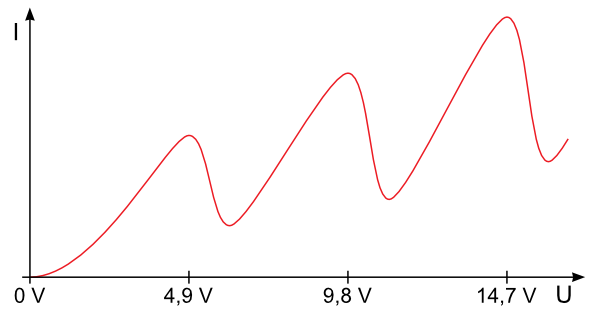
\includegraphics{theoKurve}
\caption{Theoretisch erwareter Verlauf des Anodenstromes für eine Hg-Röhre von \cite[12.03.2015,16 Uhr]{lp22}}
\label{fig:theoKurve}
\end{figure}
Man tut dies, in dem man Elektronen mit einer Glühkathode emmitiert und zunächst von der Glühwendel mit einer Raumladungsspannung leicht beschleunigt.
Die hauptsächliche Beschleunigung findet jedoch erst zwischen den zwei Gittern durch die Beschleugigungsspannung $U_1$ statt.
Nachdem die Elektronen das zweite Gitter durchquert haben, werden sie von einer kleineren Bremsspannung erneut abgebremst.
Dies wird gemacht, damit nur Elektronen mit einer genügend hohen Energie die Anode erreichen können.

Die Elektronen haben nach einer Beschleunigung mit der Spannung $U$ eine Energie von 
\begin{align}
E=e\cdot U\label{eq:EU}
\end{align}
wobei nach \cite[S. 32]{demtroeder2} $e = \SI{1.6022e-19}{\coulomb}$ die Elementarladung darstellt.

Sind die Elektronen nun so stark beschleunigt, dass sie gerade die Atome anregen können, so hat die Wellenlänge des ausgesandten Lichts gerade die Frequenz
\begin{align}
e\cdot U=h\cdot \nu \label{eq:eUhnu}
\end{align}

Die nun verlangsamten Elektronen haben zunächst zu wenig Energie um die Bremsspannung zu überwinden.
Daher kommt zunächst kaum ein Stromfluss zustande (nur diejenigen Elektronen, welche keine Geschwindigkeit verloren haben kommen durch).
Ist die Strecke in der Röhre jedoch noch lang genug nach dem Stoß, so können die Elektronen wieder soweit beschleunigt werden, dass sie erneut die kritische Schwelle überschreiten können.


\section{Durchführung}
\label{sec:durchfuehrung}
\begin{figure}[h]
\centering
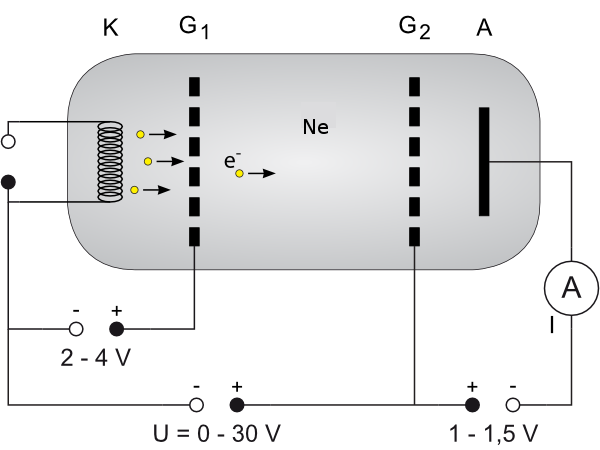
\includegraphics{RoehreNe}
\caption{Aufbau des Versuchs, modifiziert nach \cite[12.03.2015,16 Uhr]{lp22}}
\label{fig:aufbau}
\end{figure}
In Abb. \ref{fig:aufbau} ist der Aufbau des Franck-Hertz-Versuches dargestellt.
Hierbei werden die Neonatome nicht durch Photonen, sondern durch freie Elektronen angeregt.
Diese werden durch den glühelektrischen Effekt (s. Protokoll 12 - spezifische Elektronenladung) von einer Glühwendel emmitiert werden und dann mit einer elektrischen Spannung beschleunigt werden.
Zunächst werden Heizspannung $U_H$, Raumladungsspannung $U_3$ und Anodenbremsspannung $U_2$ wie auf dem Gerät vermerkt eingestellt.
Die Beschleunigungsspannung wird zu Beginn auf $0\si\volt$ gesetzt.
Obwohl in der Praktikumsanleitung keinerlei Hinweise auf ein Vorheizen des Neon-Aufbaus zu finden war, haben sich unsere Messwerte zu Beginn noch verändert, so dass dies sinnvoll zu sein scheint.

Um die Messung durchzuführen, ohne jedes mal zwischen den verschiedenen Ansichten des Steuerkastens hin- und herzuschalten, wird ein Voltmeter genutzt, um eine Ausgangsspannung zu vermessen, die proportional zum Anodenstrom ist.
Diese soll nun in Schritten $\Delta U_1=0.5\si\volt$ der Beschleunigungsspannung vermerkt werden.
Dies geschieht, bis $U_1=90\si\volt$ erreicht hat, oder eine Bogenentladung in der Röhre stattfindet.
Sollte dies geschehen, so schaltet sich das Steuergerät ab und die Messwerte nach erneutem Anschalten sind nicht mehr konsistent mit den vorher aufgenommenen.
Es ist daher davon abzusehen, testweise die Spannung zu erhöhen.

Bei der Durchführung kann man ab und zu einem Blick auf die Röhre werfen, da nach dem ersten Einbruch des Stromes dort eine schwach leuchtende Scheibe zu sehen ist.
Mit steigender Energie der Elektronen sind mehr Scheiben erkennbar, da diese wieder genügend beschleunigt werden um erneut Atome anzuregen.
Dies ist bei dem Aufbau mit der \chemical{Hg}-Röhre nicht der Fall, da dort die Emmision nicht im sichtbaren Bereich liegt.

\section{Auswertung}
\label{sec:auswertung}
\begin{figure}[h]
\centering
% GNUPLOT: LaTeX picture with Postscript
\begingroup
  \makeatletter
  \providecommand\color[2][]{%
    \GenericError{(gnuplot) \space\space\space\@spaces}{%
      Package color not loaded in conjunction with
      terminal option `colourtext'%
    }{See the gnuplot documentation for explanation.%
    }{Either use 'blacktext' in gnuplot or load the package
      color.sty in LaTeX.}%
    \renewcommand\color[2][]{}%
  }%
  \providecommand\includegraphics[2][]{%
    \GenericError{(gnuplot) \space\space\space\@spaces}{%
      Package graphicx or graphics not loaded%
    }{See the gnuplot documentation for explanation.%
    }{The gnuplot epslatex terminal needs graphicx.sty or graphics.sty.}%
    \renewcommand\includegraphics[2][]{}%
  }%
  \providecommand\rotatebox[2]{#2}%
  \@ifundefined{ifGPcolor}{%
    \newif\ifGPcolor
    \GPcolortrue
  }{}%
  \@ifundefined{ifGPblacktext}{%
    \newif\ifGPblacktext
    \GPblacktexttrue
  }{}%
  % define a \g@addto@macro without @ in the name:
  \let\gplgaddtomacro\g@addto@macro
  % define empty templates for all commands taking text:
  \gdef\gplbacktext{}%
  \gdef\gplfronttext{}%
  \makeatother
  \ifGPblacktext
    % no textcolor at all
    \def\colorrgb#1{}%
    \def\colorgray#1{}%
  \else
    % gray or color?
    \ifGPcolor
      \def\colorrgb#1{\color[rgb]{#1}}%
      \def\colorgray#1{\color[gray]{#1}}%
      \expandafter\def\csname LTw\endcsname{\color{white}}%
      \expandafter\def\csname LTb\endcsname{\color{black}}%
      \expandafter\def\csname LTa\endcsname{\color{black}}%
      \expandafter\def\csname LT0\endcsname{\color[rgb]{1,0,0}}%
      \expandafter\def\csname LT1\endcsname{\color[rgb]{0,1,0}}%
      \expandafter\def\csname LT2\endcsname{\color[rgb]{0,0,1}}%
      \expandafter\def\csname LT3\endcsname{\color[rgb]{1,0,1}}%
      \expandafter\def\csname LT4\endcsname{\color[rgb]{0,1,1}}%
      \expandafter\def\csname LT5\endcsname{\color[rgb]{1,1,0}}%
      \expandafter\def\csname LT6\endcsname{\color[rgb]{0,0,0}}%
      \expandafter\def\csname LT7\endcsname{\color[rgb]{1,0.3,0}}%
      \expandafter\def\csname LT8\endcsname{\color[rgb]{0.5,0.5,0.5}}%
    \else
      % gray
      \def\colorrgb#1{\color{black}}%
      \def\colorgray#1{\color[gray]{#1}}%
      \expandafter\def\csname LTw\endcsname{\color{white}}%
      \expandafter\def\csname LTb\endcsname{\color{black}}%
      \expandafter\def\csname LTa\endcsname{\color{black}}%
      \expandafter\def\csname LT0\endcsname{\color{black}}%
      \expandafter\def\csname LT1\endcsname{\color{black}}%
      \expandafter\def\csname LT2\endcsname{\color{black}}%
      \expandafter\def\csname LT3\endcsname{\color{black}}%
      \expandafter\def\csname LT4\endcsname{\color{black}}%
      \expandafter\def\csname LT5\endcsname{\color{black}}%
      \expandafter\def\csname LT6\endcsname{\color{black}}%
      \expandafter\def\csname LT7\endcsname{\color{black}}%
      \expandafter\def\csname LT8\endcsname{\color{black}}%
    \fi
  \fi
  \setlength{\unitlength}{0.0500bp}%
  \begin{picture}(7200.00,5040.00)%
    \gplgaddtomacro\gplbacktext{%
      \csname LTb\endcsname%
      \put(682,704){\makebox(0,0)[r]{\strut{} 0}}%
      \put(682,1156){\makebox(0,0)[r]{\strut{} 1}}%
      \put(682,1609){\makebox(0,0)[r]{\strut{} 2}}%
      \put(682,2061){\makebox(0,0)[r]{\strut{} 3}}%
      \put(682,2513){\makebox(0,0)[r]{\strut{} 4}}%
      \put(682,2966){\makebox(0,0)[r]{\strut{} 5}}%
      \put(682,3418){\makebox(0,0)[r]{\strut{} 6}}%
      \put(682,3870){\makebox(0,0)[r]{\strut{} 7}}%
      \put(682,4323){\makebox(0,0)[r]{\strut{} 8}}%
      \put(682,4775){\makebox(0,0)[r]{\strut{} 9}}%
      \put(814,484){\makebox(0,0){\strut{} 0}}%
      \put(1670,484){\makebox(0,0){\strut{} 10}}%
      \put(2525,484){\makebox(0,0){\strut{} 20}}%
      \put(3381,484){\makebox(0,0){\strut{} 30}}%
      \put(4236,484){\makebox(0,0){\strut{} 40}}%
      \put(5092,484){\makebox(0,0){\strut{} 50}}%
      \put(5947,484){\makebox(0,0){\strut{} 60}}%
      \put(6803,484){\makebox(0,0){\strut{} 70}}%
      \put(176,2739){\rotatebox{-270}{\makebox(0,0){\strut{}$U \propto I_A$ [V]}}}%
      \put(3808,154){\makebox(0,0){\strut{}$U_1$ [V]}}%
    }%
    \gplgaddtomacro\gplfronttext{%
      \csname LTb\endcsname%
      \put(2134,4602){\makebox(0,0)[r]{\strut{}Messwerte}}%
    }%
    \gplbacktext
    \put(0,0){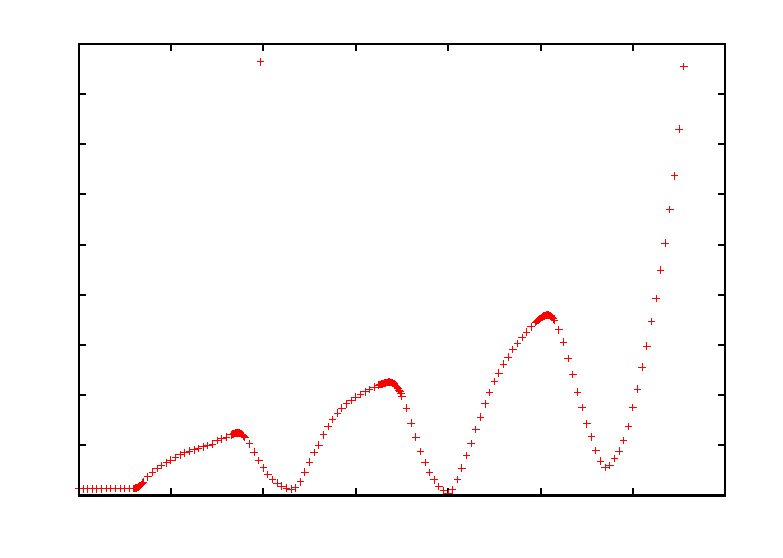
\includegraphics{messwerte}}%
    \gplfronttext
  \end{picture}%
\endgroup

\caption{Messwerte}
\label{fig:messwerte}
\end{figure}
In Abb. \ref{fig:messwerte} sind die Messwerte aufgetragen.
Die eingezeichneten Fehler betragen $(0.02+1\%)\si{\volt}$, da die Schwankungen in Bereichen von $0.02\si\volt$ liegen und das verwendete Messgerät eine Genauigkeit von $1\%$ besitzt.

\subsection{Maxima}
Die in Abb. \ref{fig:geraden} eingezeichneten Geraden

\section{Diskussion}
\label{sec:diskussion}

\bibliography{literatur}
\bibliographystyle{babalpha}
\end{document}
